\documentclass
[english,a4paper]{article}




\usepackage{graphicx}
\usepackage{cite}

\begin{document}
\title{Distributed File System for Storage of Document with Gifford
  Read/Write Constraints}
\author{Mark Wagy}

\maketitle

\newpage
% ============================================================
% ============================================================
\section{Design Document: System Design}

\subsection{Design Overview}
For this project I have implemented a distributed file system that
serves a document and replicates that document between file server
nodes. It allows the user to interact directly through the client to
read and write to a shared and 
versioned document that exists on the distributed data store. This
document is replicated throughout the file system on multiple file
system nodes. When the user either requests a write or a read, their
request is put into a queue of read/write requests. When the
read/write request queue is ready to implement the requested action,
a quorum of file system nodes are elected at random according to a
defined number in a configuration file. If the number of read and
write file server nodes obeys the Gifford Read/Write constraints \cite{gifford_weighted_1979}

The system consists of a set of clients, a set of file servers and a
``Collector''. The clients are the point of interaction with the
system. The file servers are the entities that store the document. The
collector is the point for the client to make requests and the entity
that controls the election of read and write quora for the sake of
distributed reads and writes to the file servers.

\subsection{Write constraints and the \emph{Collector}}
Each component in the system needs to know where the Collector resides
(its IP address and port number) since the Collector handles both the
request queue and the assignment of the port numbers that the file
server nodes use. The Collector is also responsible for the
enforcement of the Gifford read/write constraints. When the client
requests either a read or write, the Collector assures that the number
of reads and the number of writes fall within the requirements that
the number of writes exceeds half of the total number of file server
nodes nodes for a write to take place and when a read takes place it
ensures that the number of read nodes and the number of write nodes is
greater than the total number of file server nodes.

\subsection{Language and technical details}
The system is implemented in the Java programming language and uses
Remote Method Invocation (RMI) to handle the interaction between all
components of the system. 

The \emph{Collector} class - which directly represents the Collector
abstraction per the requirements for the assignment - maintains a
\emph{RequestQueue} object. This \emph{RequestQueue} is a child class
of a Java \emph{Queue}, which maintains a set of \emph{Request}
values. The \emph{Request} object contains an enumerated type of
either \emph{Read} or \emph{Write} to maintain whether the request
itself is either a read or a write request. This \emph{Request} type
also maintains a time, number and value fo the request. The value is
used to store the \emph{String} value of the write when a request is
of the \emph{write} type. The \emph{RequestQueue} simply has the
methods to either add a \emph{Request} or get a \emph{Request}.

When the \emph{Collector} gets a read or write request, it first
returns a request number to the client that is calling it. The client
then uses this number to gather the results of the request when the
Collector has determined that that particular request was the next
request to be fulfilled. If the request is a read request, a
\emph{String} of the contents of the file system is returned and if
the request was a write request, a boolean value indicating the
success (or lack thereof) of the write to the distributed file system.

The file server is represented by the \emph{File Server} class. It
basically maintains a Serialized version of a document - the
\emph{Document} class. The \emph{Document} class maintains a String,
which is the document that is read and written, as well as a version
number that increments each time the \emph{Document} instance's
\emph{String} value changes. 

\subsection{The \emph{Client} and user interaction}
The \emph{Client} abstraction is the user interface to the
system. It takes the argument of where to find the \emph{Collector}
instance - just like the \emph{FileServer} object does. There are two
main ways of interacting with the client: the user can invoke the
``interactive'' mode of using the client and the user can use the
client purely from the command line, passing in the read and write
parameters to the program to execute a single read or write request
(more detail about the use of the interaction of the user with the
client is the the User Document).

\newpage
% ============================================================
% ============================================================
\section{User Document: System Usage}

\subsection{Building the System}

To build the system, Java must be installed and the Ant build system
must also be installed on the user's machine. Then the user must type:

\begin{verbatim}
ant jar
\end{verbatim}


\subsection{Basic System Startup}

\subsubsection{Single Command Startup}
Scripts are provided for system startup. The main script, ``run.sh''
is provided as a means to start the entire system with just one
command. This starts three clients, a collector and five file
servers. The user is prompted at each step to start the components of
the system in the proper order: first the Collector, then the File
Servers and then the Client. 

\begin{verbatim}
WHen collector has finished starting, hit [Enter]...
\end{verbatim}

When the collector has finished, it will display a message indicating
that it has finished:

\begin{verbatim}
INFO [main] - Collector finished with startup
\end{verbatim}

At this point the user must hit \emph{Enter} to continue with the
startup of the File Servers (as indicated by the similar message as
indicated above for the Collector).

When the five file servers have displayed the message as follows:

\begin{verbatim}
INFO [main] - File server at <port number> finished with startup
\end{verbatim}

Then the user should hit \emph{Enter} once more for the Client to
start itself. At this stage, the user will be presented with the
Client's \emph{Interactive Mode} menu (more details below).

\subsubsection{Multiple Command Startup}
Alternatively, separate scripts can be used to start any
combination of numbers of clients and file servers at any
location. These scripts are ``run\_clients.sh'',
``run\_fileservers.sh'' and ``run\_collector.sh''.

The components of the system must be started in the order:

\begin{enumerate}
\item{Collector}
\item{File Servers}
\item{Client}
\end{enumerate}

To start the Collector, one must only type:

\begin{verbatim}
./run_collector
\end{verbatim}j

If the system is to be started up on multiple machines, the location
of the collector (its IP address and its port number) must be noted
and provided as arguments to the Client and File Server startup
programs (this can be done within the ``run\_fileservers\.sh'' and
``run\_client\.sh'' scripts under the environment variable values
\emph{COLLECTOR\_IP} and \emph{COLLECTOR\_PORT}).

The File Server startup script takes an argument of the number of file
servers to start on that particular machine. For example, if you want
to start ten file servers on that machine, you would type:

\begin{verbatim}
./run_fileservers.sh 10
\end{verbatim}


\subsection{Client Interactive Mode}
The clients are the processes with which the user interacts. The two mandatory arguments that are needed for startup of the client are the IP address and port number of the Collector. Upon starting a client, the user is presented with a menu of options as follows:

\begin{verbatim}
Would you like to:
(r) Request a read
(w) Request a write
(f) Query file servers through Collector
(q) Quit
\end{verbatim}

This is the ``interactive mode''  of the client. The choices are
self-explanatory: the user can request a read or write to the file
system document, can quit the program or can do a query of the
information of each file server that has been started in the system
(through the Collector). The latter action prints the IP address, port
and version number of the document that is stored on that particular
file server. Note that if multiple clients are desired, they must be
fed the appropriate IP address and port of where the collector is
running. By default, there are three separate collector instances
listening at the base port that the collector is defined on and two
other ports - one higher than the base port and two higher than the
base port, respectively. For example, if the base port that the
collector is running on is 44555, then the collector will also be
listening on ports 44556 44557 for additional client instances.

\subsection{Client Batch Mode}
An alternative way to use the client is in a non-interactive way. If one would like to do a read request, an extra parameter of ``r'' is added (in addition to the Collector IP address and port number) to the command-line invocation of the client script. This will cause a single read operation to be performed by the client on the file system. Similarly, a ``w'' along with a string (in double quotes) to write are passed as added arguments to the client and a single write operation of the given string is performed on the distributed file system. This type of usage of the client allows the user to do batch read and write operation requests to the file system from the command line.

\subsection{Test Scripts}
Test scripts are provided as a means for testing multiple read and
write requests. Both a ``Read-Heavy'' and a ``Write-Heavy'' script are
provided to test the system. To invoke these scripts, one must have
already started the \emph{Collector} as well as the number of
\emph{FileServer} objects that are desired for the tests. The provided
test scripts are only invocations of the ``Batch Mode'' of the client
called multiple times. The actual contents of the tests
that are performed in these scripts is detailed in the \emph{Testing
  Description} portion of this document.

\subsubsection{Read-Heavy Tests}
To invoke the ``Read-Heavy Test'' script, go to the base directory of
the project, and type:

\begin{verbatim}
./test_read_heavy.sh
\end{verbatim}

\subsubsection{Write-Heavy Tests}
To invoke the ``Write-Heavy Test'' script, go to the base directory of
the project, and type:

\begin{verbatim}
./test_write_heavy.sh
\end{verbatim}

\newpage
% ============================================================
% ============================================================
\section{Testing Description: System Tests}

A series of tests were performed to verify the correctness of the
system. Some of these tests were included with the packages for easy
reproduction (see the \emph{test\_read\_heavy\.sh} and
\emph{test\_write\_heavy\.sh} scripts). Some of the tests were
performed to determine any patterns in whether a particular
configuration of the number of nodes that were used in both the read
quorum and the write quorum of file servers arose as the result of
``ready-heavy'' and ``write-heavy'' combinations of read and write
requests as detailed below.

\subsection{Performance Evaluation}

A series of tests were performed to assess the behavior of various
combinations of read and write quorums given a fixed size of file
server nodes to store a document in the distributed file store
system. 

Scripts were created to be tested for the system timing of
write and reading to the file store. The timing of the scripts was
taking from the beginning of invoking the script in question to the
time of completion using the \emph{time} command that is available in
Linux and OSX environments.

\subsubsection{Read-Heavy Workloads}

A so-called ``read-heavy'' workload was generated to test the time
that it takes the distributed document system to have a significantly
higher amount of read requests to the number of write requests that
the batch-style client performs on the system. 

The read-heavy test workload consists of reading and writing words
in the following sequence (with R representing reads and W
representing writes): 

\begin{verbatim}
R10, W1, R40, W4, R10, W5, R40, W4. 
\end{verbatim}

In total, this results in 100 reads and 14 writes. This is the same
total number of reads and writes as for the write-heavy workload
below, which allows us to have an ``apples to apples'' comparison
between the two types of workloads.

The initial hypothesis in performing a read-heavy workload on the
distributed system would be that the time that it takes to finish the
workload would be lower in general than the write-heavy workload
scenario, since the need for updating all file server nodes would
cause more of a detrimental performance impact on the system than
simply reading from the most updated copy of the document in the
distributed file system as in the case for performing a read
operation.

Additionally, it would not be expected that the number of  either the
write quorum or the read quorum would have a significant impact on the
performance of the distributed document file system - we would expect
that the timing-readings would be relatively flat.

The result of the experiment are summarized in the following table:

\begin{center}
\begin{tabular}{| c | c | c | c | c | c | c}
\hline
\emph{N} & \emph{Nw} & \emph{Nr} & \emph{system time}\\ \hline
5 &5 & 1 & 12.824 \\ \hline
5 &5 & 2 & 12.699 \\ \hline
5 &5 & 3 & 12.757 \\ \hline
5 &5 & 4 & 12.335 \\ \hline
5 &5 & 5 & 12.253 \\ \hline
5 &4 & 5 & 12.306 \\ \hline
5 &3 & 5 & 12.358 \\ \hline
\end{tabular}
\end{center}

\subsubsection{Write-Heavy Workloads}

Similar to the idea of the ``read-heavy'' workload discussed
previously, a ``write-heavy'' workload was generated to evaluate the
performance of the distributed file system in a situation where many
write requests were committed to the distributed document.

The write-heavy workload consists of a test of reading and writing
words in the following sequence (with R representing reads and W
representing writes): 

\begin{verbatim}
W10,R1, W40, R4, W10, R5, W40, R4
\end{verbatim} 

In total, as in the case of the ``write-heavy'' workload, this gives
us 100 writes and 14 reads. 

The initial hypothesis would be that we would see more of an impact of
the number of values that are elected in the quora than in the
``read-heavy'' workload example. This would be due to the fact that,
as the document in the distributed file system is changed due to write
requests, the number of updates to documents in the file store would
need to be spread and committed to the replicated file server nodes.

The result of the experiment
are summarized in the following table and plot:

\begin{center}
\begin{tabular}{| c | c | c | c | c | c | c}
\hline
\emph{N} & \emph{Nw} & \emph{Nr} & \emph{system time (s)}\\ \hline
5 &5 & 1 & 12.707 \\ \hline
5 &5 & 2 & 12.672 \\ \hline
5 &5 & 3 & 12.429 \\ \hline
5 &5 & 4 & 12.479 \\ \hline
5 &5 & 5 & 12.400  \\ \hline
5 &4 & 5 & 12.341  \\ \hline
5 &3 & 5 & 12.493 \\ \hline
\end{tabular}
\end{center}

Plots of the relationship between the number of read file server nodes
in the quorum versus the time that it took for both the read-heavy and
the write-heavy operations to complete are shown in the below figures:

\begin{center}
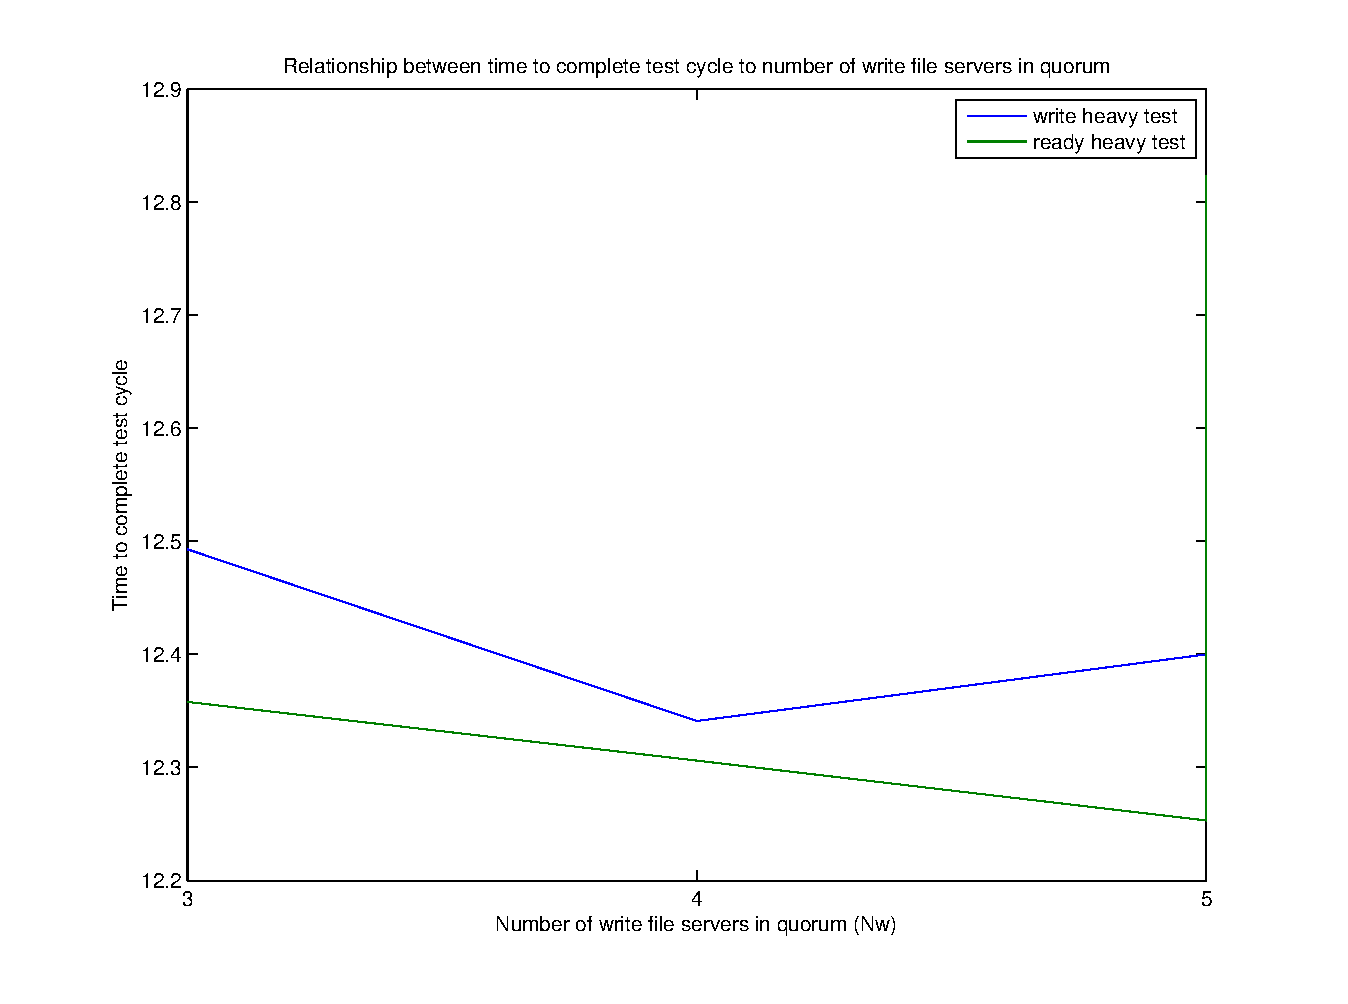
\includegraphics[scale=0.6]{write_fs_quorum} \\
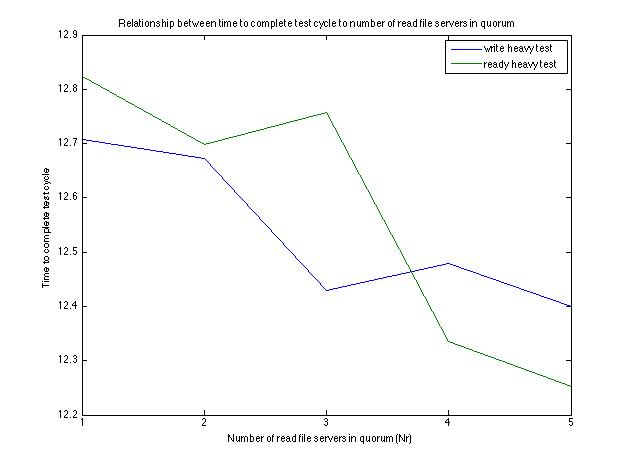
\includegraphics[scale=0.6]{read_fs_quorum}
\end{center}

We stated in the initial hypotheses that the impact of the number of file server
nodes that are used in the quora for read and write requests would be
more significant for write-heavy requests than for read-heavy
requests. From the plots, this does not appear to be the case. If it
were the case, we would see that the write-heavy requests would
consistently take more time than the read-heavy requests. While this
is the case when looking at the first plot (i.e. the blue line
representing the write-heavy requests is always above the green line
representing the read-heavy requests), it is not consistently the case in the lower
plot.

One factor that may explain this discrepancy with the initial
hypothesis is that, when performing a read request, the client prints
the contents of the document to standard-out for review of the
document itself. This printing to screen can take significantly longer
when we have a significant amount of text stored in the document and
thus obscure the actual costs of reads versus writes to the
distributed file system.

A trend that becomes apparent when looking at the values and the plots
that compare the read-heavy and write-heavy tests is that the time
that the tests take is less for more read file servers nodes that are
used in the quorum (as seen in the lower plot). This is regardless of
whether we are doing a read-heavy or write-heavy set of test
requests. This is also the case when looking at the number of
increasing number of file server write nodes in the quorum, but to a
lesser degree than that of looking at the number of read file server
nodes that are elected to the quorum.

A possible explanation for the tendency to have more read nodes in the
quorum to have a beneficial impact on the system performance would depend on the
hypothesis just mentioned that reads are a more significant sink on
the systems performance due to the time that it takes the document in
the distributed file store to be printed to standard out. If this is
in fact the case, we can say that reads have more of an impact on the
system's performance. As such, improvements to the read action of the
system would have a significant impact. An improvement on read
performance is the ability to quickly get a copy of the document that
is stored on the distributed file system, and having more designated
``read'' file server nodes in the elected read quorum allows quicker
access to the most recent version of the document in the file
store. However, if the largest impact is on the printing of the
document to the user's screen, accessing the document may have little
impact on the ability of the system to have better time performance
due to the quick access of the document itself. It is also possible
that the performance of the system was affected by other processes and
that the trend is something of a ``red herring'' - in reality there is
no such trend and the other processes on the system affected the
timing in an arbitrary manner. A more rigorous test to determine
whether this trend is, in fact, a true trend would be to run multiple,
identical such read-heavy and write-heavy scripts at different and
randomized times throughout the day. This would have the effect of
randomizing the affect of processes on the performance of the
distributed file server system. An obvious alternative would be to
assure that no other processes were running at the same time, but this
is a less feasible way to isolate the purported trend versus the
concept of just randomizing the impact of other processes on the
distributed file server system.



\newpage
\bibliographystyle{plain}
\bibliography{pa2}

\end{document}
